\subsection{Propuesta solución}

Para la concepción de la propuesta solución, fue necesario realizar un análisis por medio de una matriz morfológica. Esta es una tabla en la que se ilustran las diferentes opciones que se pueden seleccionar para la construcción de los diferentes sistemas del dispositivo. 

Dentro de ella se trazan diversas rutas de diseño a través de las cuales se van seleccionando los mecanismos necesarios y se va dando forma a un diseño conceptual del dispositivo mecatrónico.

Para este proyecto, se propone la matriz morfológica que se encuentra en el apéndice \ref{Ap:Mat_Morfo}, donde se muestran las opciones que existen para construir los diferentes sistemas de trituración, aireación, monitoreo, regulación y comunicación.
        
De esta forma, se comienzan a trazar diferentes rutas de diseño en la tabla morfológica para seleccionar cada una de las partes del diseño del sistema y así proponer diferentes modelos del sistema mecatrónico, los cuales se someten a una etapa de deliberación para poder seleccionar el que más convenga.

Los diferentes modelos que se proponen para su posterior análisis, se encuentran descritos en la tabla \ref{tab:modelosPro}.

\begin{table}[h]
    \centering
    \caption{Modelos propuestos} 
    \begin{tabular}{c|c|c|c}
    \hline
        Modulo & Modelo 1 & Modelo 2 & Modelo 3\\ \hline
        Trituración &  A & D & C\\
        Almacenamiento & B & B & B \\
        Palas de agitación & B & D & A \\
        Transmisor de movimiento motor-eje & A & D & B\\
        Medir temperatura & C & B & D \\
        Medir humedad & A & A & B \\
        Elevar la Temperatura & C & B & A \\
        Unidad de procesamiento & A & A & B\\
        Interfaz usuario - Maquina & C & D & A
    \end{tabular}
    \label{tab:modelosPro}
\end{table}

Con el proceso de selección del diseño conceptual fueron elaborados 2 bocetos diferentes que contemplan las soluciones propuestas para cada uno de los módulos y sistemas, variando solo su distribución, tal como se muestra en la imagen (Figura \ref{fg:conceptos}).

\begin{figure}[h!]
    \centering
        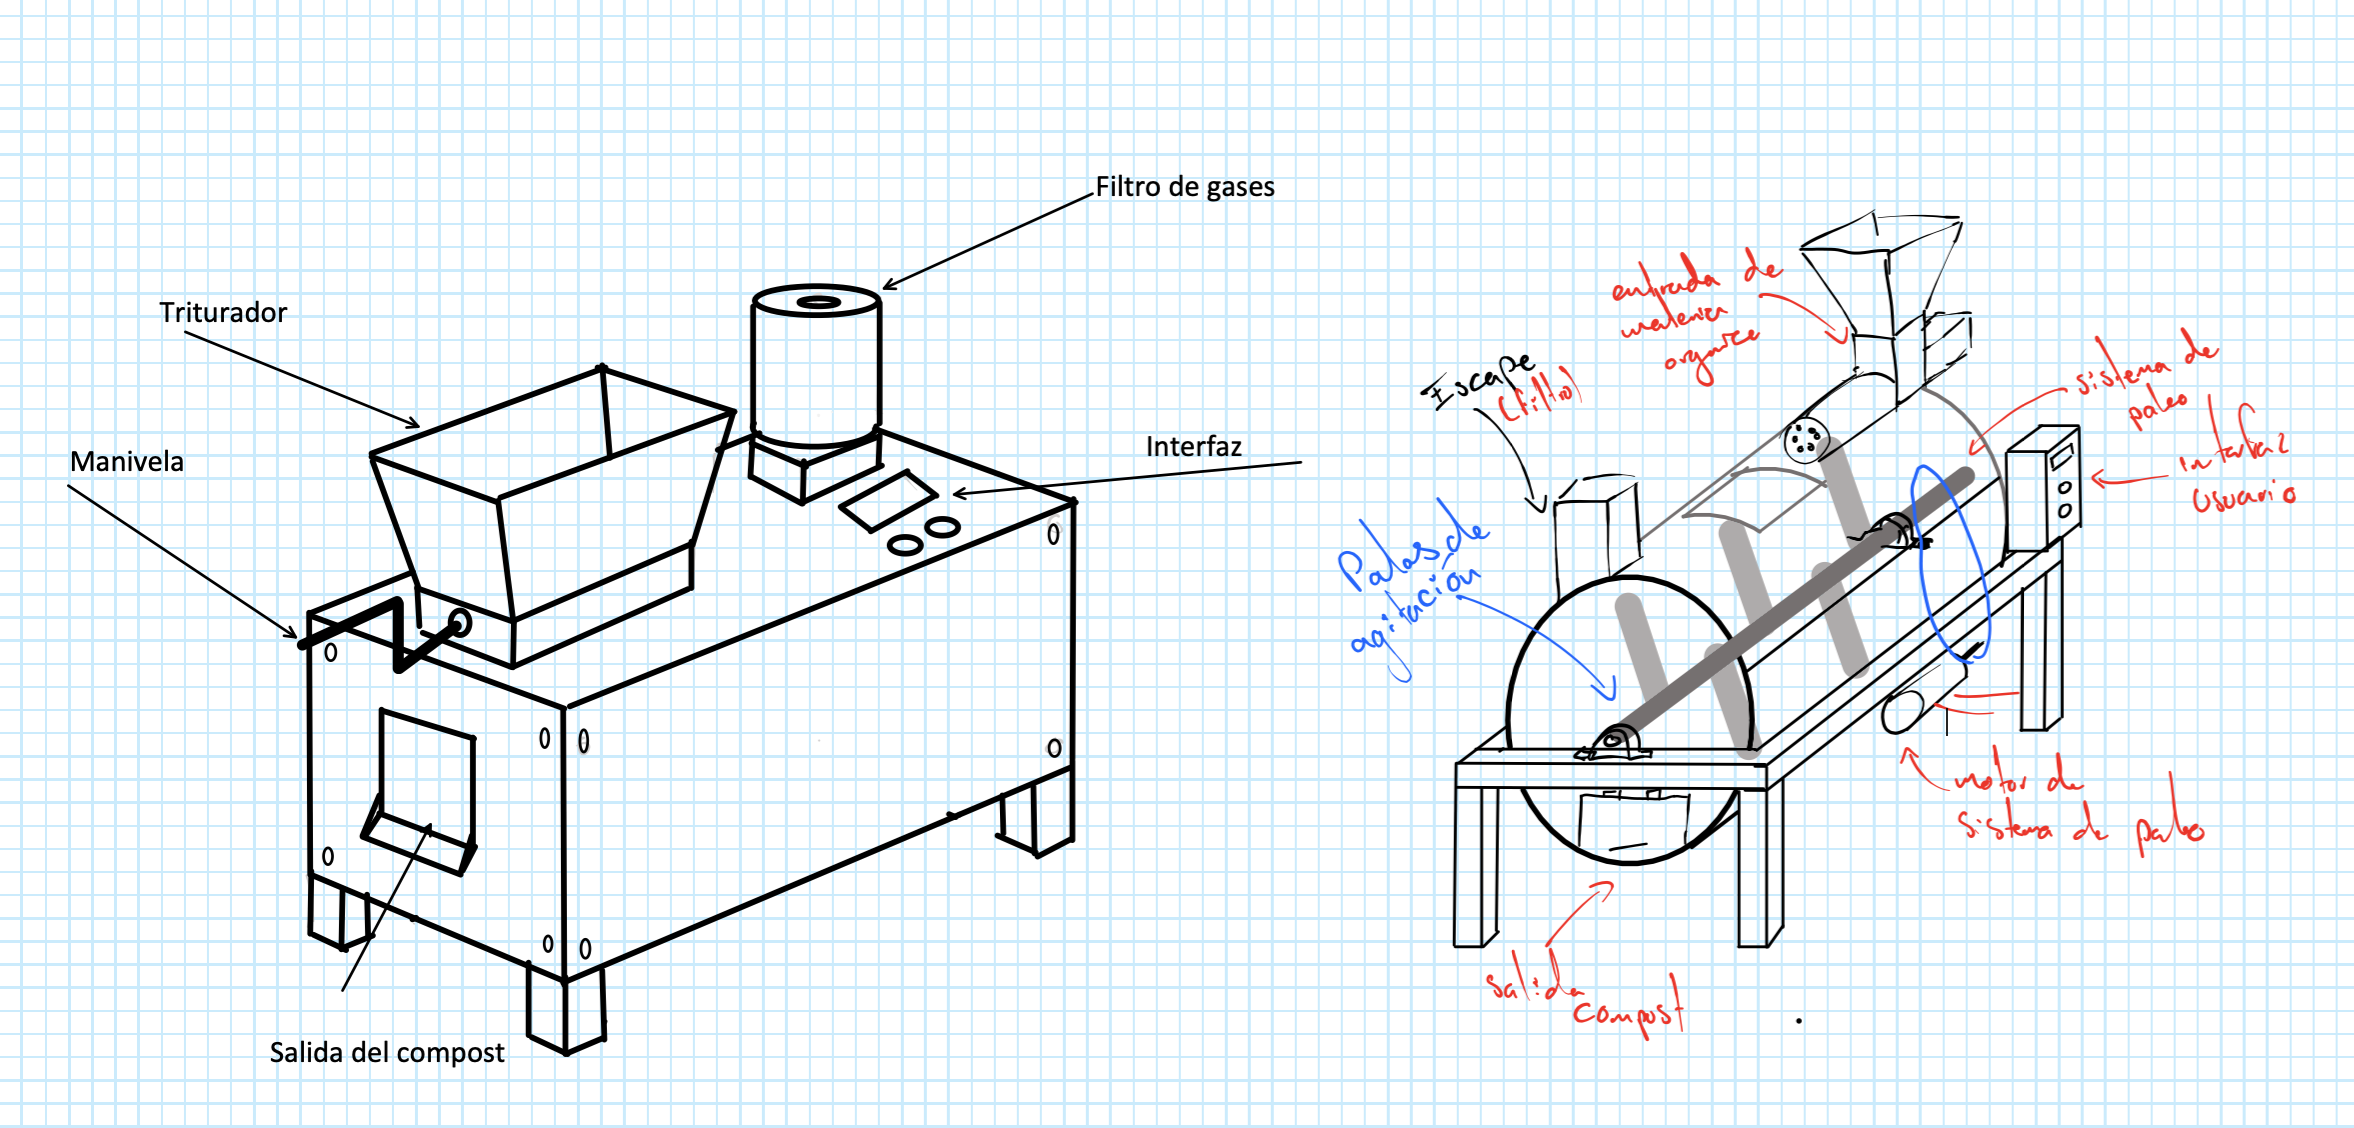
\includegraphics[scale=0.25]{images/Capitulo 3/3.2.5 Diseño Conceptual/ConceptosGenerados.png}
        \caption{Conceptos Generados}
    \label{fg:conceptos}
\end{figure}